\documentclass[tikz,border=10pt]{standalone}
\usepackage{tikz}
\usepackage{amsmath} % for \text
\usetikzlibrary{positioning}

\begin{document}
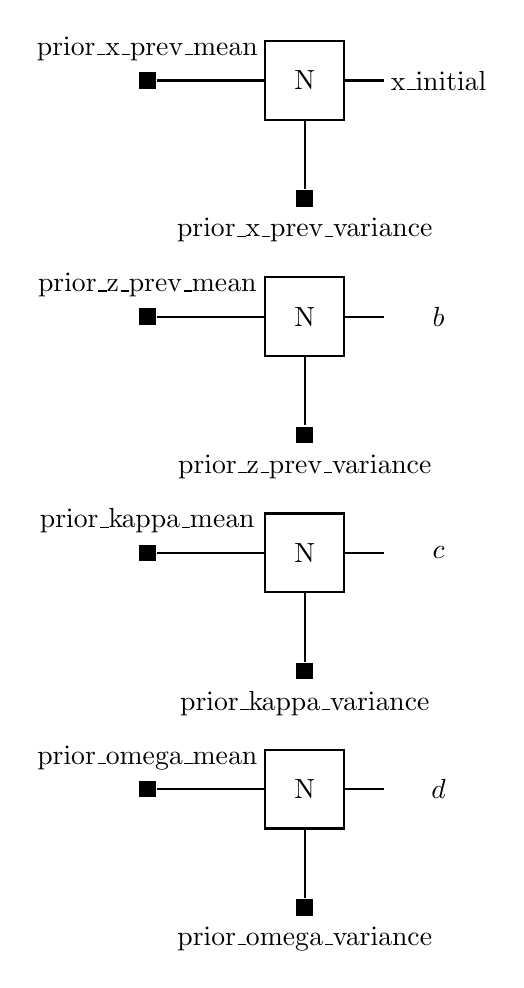
\begin{tikzpicture}[x=1cm, y=1cm,
    thick,
    % --- Styles ---
    factorNode/.style={
      fill=black,
      rectangle,
      minimum size=6pt,
      inner sep=0pt
    },
    normalBlock/.style={
      draw,
      rectangle,
      minimum width=1cm,
      minimum height=1cm,
      align=center
    }
]

%=====================
% Row A: for "x_initial"
%=====================
\node[factorNode, label=above:{$\text{prior\_x\_prev\_mean}$}] (meanA) at (0,0) {};
\node[normalBlock] (normA) at (2,0) {N};
\node[factorNode, label=below:{$\text{prior\_x\_prev\_variance}$}] (varA) at (2,-1.5) {};
\node at (3.7,0) {$\text{x\_initial}$};
\draw (meanA) -- (normA);
\draw (normA) -- (3,0);
\draw (normA) -- (varA);

%=====================
% Row B: for variable "b"
%=====================
\node[factorNode, label=above:{$\text{prior\_z\_prev\_mean}$}] (meanB) at (0,-3) {};
\node[normalBlock] (normB) at (2,-3) {N};
\node[factorNode, label=below:{$\text{prior\_z\_prev\_variance}$}] (varB) at (2,-4.5) {};
\node at (3.7,-3) {$b$};
\draw (meanB) -- (normB);
\draw (normB) -- (3,-3);
\draw (normB) -- (varB);

%=====================
% Row C: for variable "c" with kappa priors
%=====================
\node[factorNode, label=above:{$\text{prior\_kappa\_mean}$}] (meanC) at (0,-6) {};
\node[normalBlock] (normC) at (2,-6) {N};
\node[factorNode, label=below:{$\text{prior\_kappa\_variance}$}] (varC) at (2,-7.5) {};
\node at (3.7,-6) {$c$};
\draw (meanC) -- (normC);
\draw (normC) -- (3,-6);
\draw (normC) -- (varC);

%=====================
% Row D: for variable "d" with omega priors
%=====================
\node[factorNode, label=above:{$\text{prior\_omega\_mean}$}] (meanD) at (0,-9) {};
\node[normalBlock] (normD) at (2,-9) {N};
\node[factorNode, label=below:{$\text{prior\_omega\_variance}$}] (varD) at (2,-10.5) {};
\node at (3.7,-9) {$d$};
\draw (meanD) -- (normD);
\draw (normD) -- (3,-9);
\draw (normD) -- (varD);

\end{tikzpicture}
\end{document}
